\documentclass{report}

\usepackage{xeCJK}
% \usepackage[left=1in, right=1in, top=1in, bottom=1in]{geometry}
\usepackage{hyperref}
\usepackage{natbib}
\usepackage{pdfpages}
\usepackage{graphicx}
\usepackage{float}
\usepackage[top=1.5in, bottom=1.5in, left=1.5in, right=1.5in]{geometry}

\title{Final Report: A Multimedia Information Retrieval Database System}
\author{Liuyang Wang \texttt{lw2635}, Zhixuan Wang \texttt{zw2335}, Zihang Chen \texttt{zc2324}}

\begin{document}
\maketitle
\tableofcontents

\chapter{Overview}

In this document, we would like to elaborate on a multimedia information retrieval database system which retrieves related visual/acoustic information according to the style of multimedia or the users' psychological perceptions about these multimedia objects.

Typical visual database requires users to be familiar with the query system of their own, i.e., they have their own language for query. However, in this system we proposed, users will query in the database with an audio file (e.g. MP3 or OGG) as input for video clips that fits the input than other. Users can also do the query vice versa. Then the system will use various visual/acoustic features and some interconnections between them, along with a machine learning process, to try to identify queried subjects. More on how such retrieval is done will be explained later in this proposal.

When it comes to database population, one way is to evaluate the style of videos and audio and to score each of the objects according to multiple criteria, such as ``adorable'', or ``psychedelic''. The scores will be in a range of $0.0$ to $1.0$. In other words, each object will receive a vector of scores. A machine learning process will be used to fit these scores to the extracted features.

\section{Typical Use Cases}

\begin{itemize}
\item Given a piece of music, find in the database the video clips that best fit the music in the aspects of, for instance, rhythm, the emotions expressed, etc. We regard this video as a good example: \url{https://www.youtube.com/watch?v=hBVMVEsyJEE} (The title means ``Goodbye, Heaven''.) In other words, we think that if someone uses the music in this video as input, an ideal query result would be this video clip.
\item Given a video clip, find in the database the pieces of music that best fit the video clip in the aspects of, for instance, emotions/feelings, style, etc. This is exactly the opposite query regarding the first use case. Here we give another good example of such ``fit'': \url{https://www.youtube.com/watch?v=jN-snGdlzSI}.
\item Given a vector of scores, find in the database the related music and video clips that fit the score vector.
\end{itemize}

We consider the above two example videos are good fits to their respective audios because they both are merely animations with artificial shapes and simple colors that can be easily detected and obvious video structures that matches the rhythm and melody of the respective music. We consider this video \url{http://www.nicovideo.jp/watch/sm16068939} (login required, or watch it here \url{https://www.youtube.com/watch?v=2iQKFNYofD0}) to be not so good an example of what the system can query, since it is actually a tiny plotted movie that mostly relates to the lyrics of the song. It is impossible to see if this video clip is a good fit for certain piece of music without actually understanding what is happening in it.

\section{Limitations}

Since this project is only a preliminary demonstration on the combination of computer vision/audition, machine learning and database systems, we won't use many sophisticated visual/acoustic features, nor will we try to implement our system in such a way that it really ``understands'' all the multimedia information in the way human beings do. We want the system to be as simple as possible, yet quite extensible to be able to easily add new ability to it. More on the approach we will be using is discussed in the next section.

\chapter{Approaches and Methods}

\section{Distribution of Workloads}

Because it's a rather complicated project concerning computer vision and audition, machine learning and user experience, we would like to distribute these tasks in a modularized manner, such that a single person concentrates on one of these tasks. We all think that it's best for the project if one of us solely works on feature extraction part, another solely works on machine learning, and the last guy takes care of the rest of the project, i.e. the user interface and testing. If there were only two members of us, we would probably propose to do much less, for example, only query videos with classified tags.

The system will be implemented in the newest version of Python (Python 3.5.1) for fast prototyping, and roughly divided into 3 parts:
\begin{itemize}
\item The \textbf{infrastructure part}: this includes the client-server, web-based frontend that takes inputs from users and display the results; and the backend that maintains a database and invokes other modules as needed. (Zihang Chen) (HTML5, React.js, Pyramid, SQLite with SQLAlchemy as database driver)
\item The \textbf{computer vision and audition part}: this part will concentrate on the functions that extracts various features from video clips or audio files. (Liuyang Wang) (OpenCV, SimpleCV and librosa, etc.)
\item The \textbf{machine learning part}: this includes the module that fits the scores (or classification) to the features. (Zhixuan Wang) (scipy, sklearn, etc.)
\end{itemize}

\section{System Workflow}

The general workflows are depicted as follows\footnote{These two figures have been updated since the prototype demo to reflect the changes we made in the workflows implemented in the system.}:

\begin{figure}[H]
  \centering
  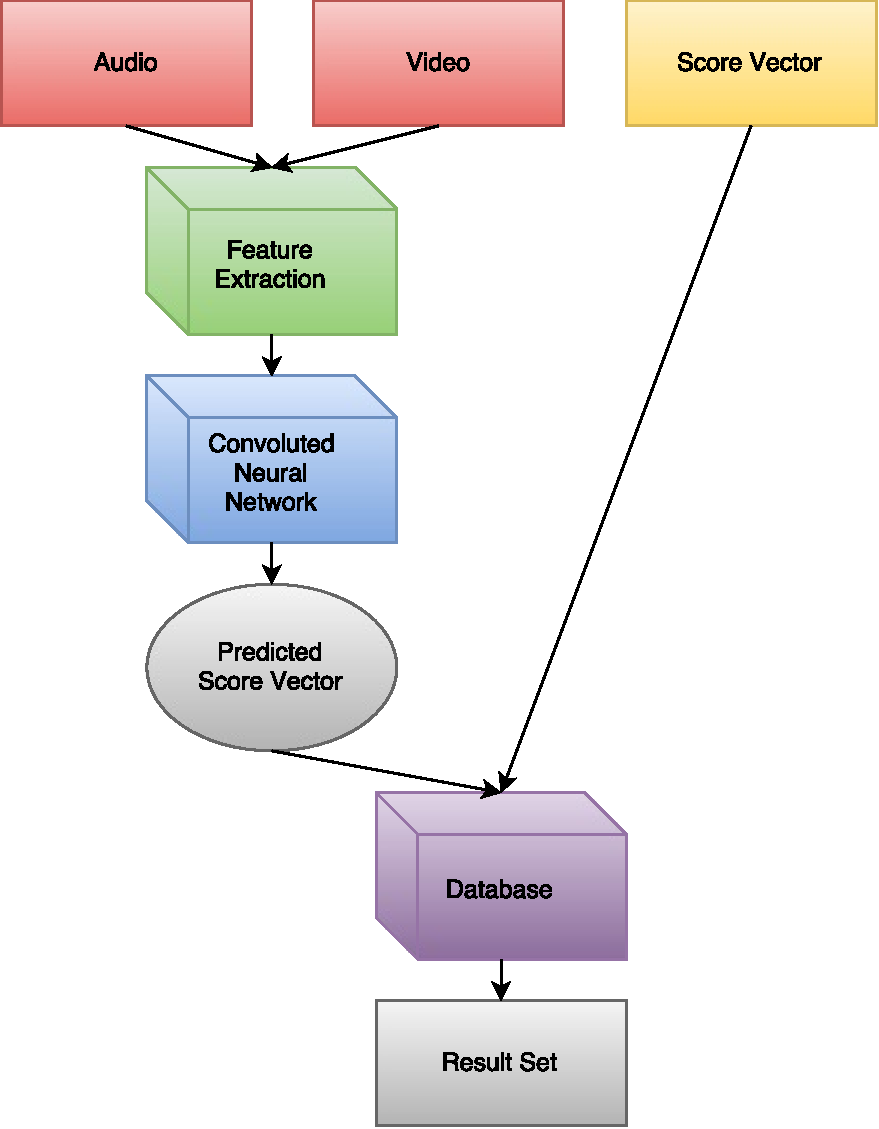
\includegraphics[scale=0.7]{vdf-query.pdf}
  \caption{Typical query workflow}
  \label{fig:qwf}
\end{figure}

The above figure depicts that users are allowed to query using audio/video files or score vectors.

\begin{figure}[H]
  \centering
  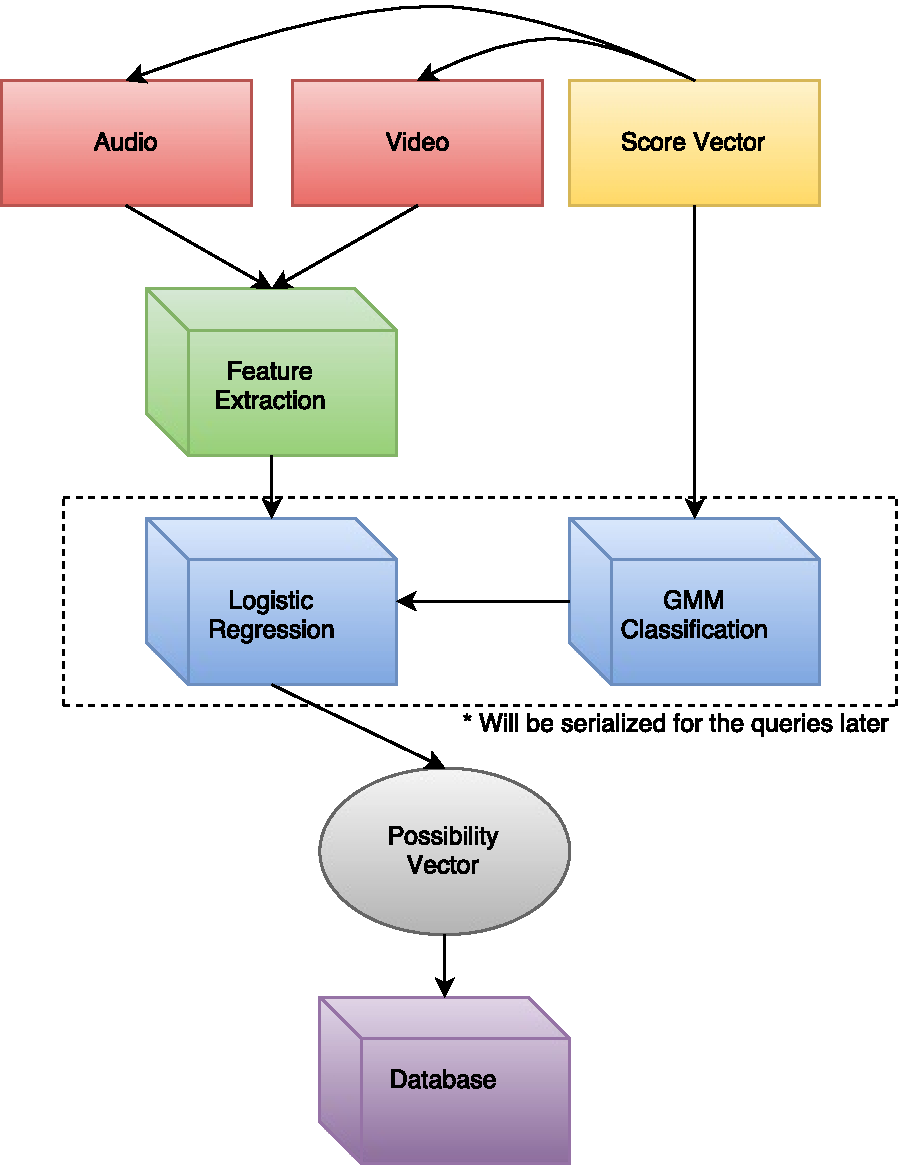
\includegraphics[scale=0.7]{vdf-pop.pdf}
  \caption{Typical database population workflow}
  \label{fig:pwf}
\end{figure}

Because of the properties of the machine learning part, i.e. they must be trained again after some new objects are submit by user. Thus, the system works best when there are many queries to the database, rather than updates.

\subsection{Development Environment}

The system is developed by three team members with three different development environment (Windows, Ubuntu and one Mac OS X), which makes it difficult for us to synchronize the development environment, especially that we experienced some difficulties installing OpenCV and it’s Python3 package on Windows. Overall, the development went smoothly.

The development environment is:
\begin{itemize}
  \item Machine: 2 high-end Windows laptops, 1 13’’ Macbook Pro
  \item Operating Systems: Windows 10, Ubuntu and Mac OS X
  \item Primarily involved software: Python 3.5, OpenCV 3.1.0, librosa 0.4.2, Pyramid 1.6.1, React.js, etc. (secondary dependencies not listed)
  \item Additionally involved hardware: none
  \item IDE: PyCharm 2016.01, WebStorm 2016.01, Visual Studio 2015
\end{itemize}

\section{System Architecture and Implementation}

The system is implemented as a Browser-Server (B/S) application, utilizing the ubiquitousness and power of browser displays and the flexibility of RESTful API. The backend (server) of the system receives RESTful API requests and invokes API of related module.

\subsection{RESTful API}

Then system currently supports three RESTful APIs:
\begin{itemize}
\item Heterogeneous Query: querying video clips with audio clips and vice versa. When dealing with this kind of requests, the system invokes feature extraction functions on the received query subject (a file object), and use the machine learning model (currently logistic regression) to predict it's possibility vector (or PV for short).

After the system procured the PV, it traverses the database, calculates and sorts the database objects by the cosine distance between the PV of the subject and the ones of the objects. Finally it replies with the sorted result set to the frontend which displays the result set in a grid.

\item Homogeneous Query: roughly the same as heterogeneous query, only that the system allows user to query objects using subjects of the same type.

\item Score vector query: user posts a score vector to the server to query something that relates to the posted score vector closely.

Note that the API for database population is removed. We realized that it is very inefficient to re-train the machine learning module very time the user uploads something new to the database. The system administrator could use the script to batch insert new clips to the database and re-train the machine learning model.

\end{itemize}

\subsection{Graphic User Interface}

The user interface is a browser-side standalone \textit{React.js} application. It is different from traditional frontend application in that it leverages the full power of Javascript to manipulate DOM node such that everything the user sees is rendered at client-side. This relieves the backend server of rendering complicated static HTML and wasting the computational power of the server machine.

The graphic user interface of the system is divided into two views. The first one is the Query View, where the user queries for multimedia clips with the file he/she dragged into the dropzone, or the score vector he/she proposed. The result of such query is displayed in grid, sorted by descending confidence (cosine distance).

The second view is the Upload View, where the user drags multiple multimeida clips into the dropzone and scores each the clips according to 8 criteria (which are \textit{Psychedelic}, \textit{Vibrant}, \textit{Happy}, \textit{Adorable}, \textit{Gloomy}, \textit{Energetic}, \textit{Romantic}, and \textit{Violent}). When the user hits \textit{Submit}, all these information will go to the server and saved into database.

\section{Feature Extraction Module}

\subsection{Acoustic Features}

To integrate audio into the machine learning part, audio clips should be represented in a way that can reveal the style or emotion of the audio clips. 

First, there are mainly two ways to represent the raw audio signal, the first way is using the raw sound wave, and the second way is divide audio signal to several frequencies and using the volume of each frequencies at each frame to depict the signal. Both ways can be easily integrated to neural network model for data training and understanding, but they are hard to be integrated into statistics machine learning method without any preprocessing. Using the whole raw data for data training will emphasize the wave pattern for data representation and retrieval, which is potentially a good approach to represent data but it may result in a relatively poor performance for data training and retrieval even when using the popular CNN method.

The feature now we are using to represent audio file the freqenucy samples sampled from audio clips with a fixed sample rate. We use the Fast Fourier Transform algorithm to extract frequecy from audio. The window size of the Fast Fourier Transform algorithm is set as two times as the frames between conjunct samples. The frequency information extracted then will be pack in to several frequency bin at each sample. The range of frequency bin is set refering to the research about human perception of audio frequency, and frequency which humans has most similar perception is packed within one bin. For each audio, we extract feature from the begining in a fixed length of the audio to guarantee that each feature has the same dimension. The feature extracted can show both the feature in time and frequency domain. We can expect this feature to provide sufficient information for the machine learning part. 

Audio feature extraction is done with Librosa, which provides audio load and FFT extraction function.

\subsection{Visual Features Extraction Implementation}

In order to distinguish different styles of videos, we have to extract the most significant features of the videos which could best represent the style of the video. It's hard to directly find a feature describing the whole video since both spatial information and temporal information are involved. Therefore we decided to extract spatial information and temporal information separately. Firstly, we divided the whole video into some segments. Within each segment, we just care about the static image information of the segment. We regarded the segment as a set of images and extracted features from it. After we extracted features of all segments, they were arranged in chronological order and regarded as the feature of the whole video.

The problem was to find a good feature to represent the video segment including a set of images. Some widely used features are descriptors of local salient points or blobs such as SIFT which represents local information well and is applied to many computer vision issues. For example, it could be used for recognizing a specific object in the image. However, Our purpose is to classify videos according to their styles. So we care more about what feelings the whole video segment could give us. Local feature descriptor seems not to be a good choice. we agreed that the color was an important information to express feelings and decided to use the color histogram as the descriptor of the video.

We implemented three different features based on the color histogram. The first one was RGB color histogram. In RGB color space, each pixel of image is represented as a 3-D vector $(r, g, b)$.For each frame $f$ of the segment, we calculated the quantized RGB color histogram ${\bf{h}_f} = [{h_{1x1x1}},...,{h_{NxNxN}}]$. For example, if the step number $N$ of each channel was 5, ${\bf{h}}$ would have a 125 dimensional vector. After that the histogram was normalized to satisfy $\sum({h_i}) = 1$.  Since a segment consisted of several images, we applied a average operator to pool all histogram into a single vector ${\bf{h}_s} = avg(\bf{h}_f)$. To speed up the feature extraction module, we did not calculate the histogram for every frame in the segment. The number of calculated frames was set according to the consideration of time cost. After the histogram feature ${\bf{h}_s}$ of all segments was generated, they were concatenated together to represent the whole video.

\begin{figure*}[htb]
\centering
\includegraphics[width=0.6\textwidth]{show.eps}
\caption{The process of generating histogram feature of a video segment.}
\end{figure*}

The second method was HSV color histogram method. It was similar to RGB color histogram method. Because HSV color space is more intuitive and perceptually than RGB color space, we believed the histogram in HSV space was better to realize our objection. Different from RGB method which the three channels were quantized equally, hue was a more significant variable here. To quantize the colors, we used more hues to quantize than saturations and values. Finally, we also got a histogram vector ${\bf{h}_s}$ to represent a segment and concatenated all vectors to represent the video.

After generating the color histogram, an important information would be discarded if we regarded the histogram as a vector directly. It was the similarity between different quantized colors. Different dimensions of the histogram vector are related to each other and should not be analyze separately in Machine Learning Module. For example, orange is more similar to red than blue. So we used a soft coding method to code histogram vector again. First of all, we randomly generated $k$ vector to represent some points $\{\bf{h}_{p1},...,\bf{h}_{pk}\}$ in HSV color space. Then for every color histogram vector ${\bf{h}_s}$ extracted from the segment. We calculated the Histogram Quadratic Distance $d^{hist}_{p,s} = (\bf{h}_s - \bf{h}_p)^t\bf{A}(\bf{h}_s - \bf{h}_p)$ as described in VisualSEEK paper bewteen ${\bf{h}_f}$ and every $\bf{h}_p$ and generated the final feature descriptor as $\bf{\mu}=[\mu_1,...,\mu_k]$, where $\mu_i$ could be calculated by
\[{\mu _{\rm{i}}} = \frac{{{e^{ - \left( {\beta  \cdot d(f,{p_i})} \right)}}}}{{\sum\limits_{j = 1}^k {{e^{ - \left( {\beta  \cdot d(f,{p_j})} \right)}}} }}\].
In this way, ${\bf{h}_s}$ was represented by its relationship $\bf{\mu}$ to $\{\bf{p}_1,...,\bf{p}_k\}$. $\bf{\mu}$ was the final descriptor of the video segment.

\begin{figure*}[htb]
\centering
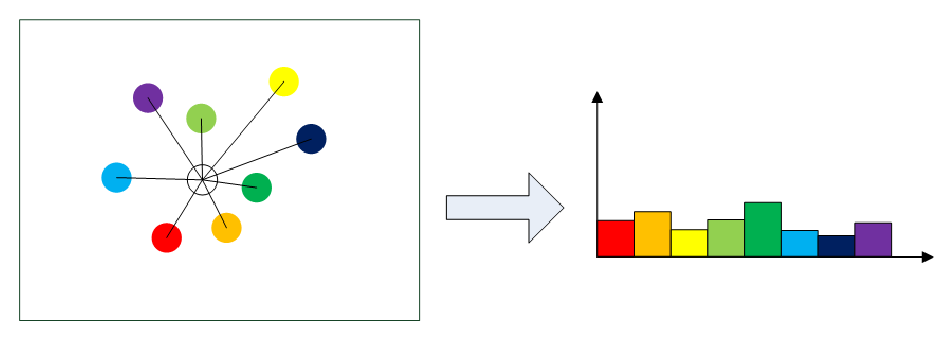
\includegraphics[width=0.6\textwidth]{coding.eps}
\caption{Soft Coding Feature.}
\end{figure*}

All three methods were written in Python3.5 with OpenCV3.1.0. The input parameters are the video's filename, time length to analyze, number of segments and some other parameters as we described. It took about 5~10 seconds to analyze a 480x360 2-minute video.

We plan to improve the performance of the histogram method in two aspects. Firstly, when calculating HSV color histogram vectors, we didn't discriminate gray colors from others. As a result, Black, white and gray are recognized as some other colors with low saturation. It might decrease the effect of our features. However, to discriminate gray colors, we must implement the calculation of histogram by ourselves in python instead of calling OpenCV functions, it might take much more time to generate the feature. The time cost might be unacceptable. Secondly, In the third method as we mentioned, we compared color histograms with some random vectors. A better solution is to cluster all kinds of histograms by clustering algorithms and use cluster centers to make the comparison. This work will be attempted after we collect more data. Meanwhile, we can try some new feature to represent the visual information like the video tempo mentioned in the recent lecture.

\section{Machine Learning Module}

In this project, we want to construct a database that can integrate audio/video clips and plaintext tags together. To build a database system that can do content-based data retrieval, we have to introduce some artificial intelligence approaches for data mining and retrieval.

To implement the data retrieval part we are going to use some exemplary well-annotated data to train the machine learning module of the database. And then generalize the data using trained machine learning module and store the result in database. When the user input comes, the database first computes the representation of the data (e.g., the scores we talked about in previous sections) via the trained machine learning module, and then find the most similar data in the database.

First, the most basic problem is that how to measure the similarity between the information with such different nature. Fortunately, the media files we can obtain often consist of both video and audio parts and even with some tag description, which will naturally provide us with the correlation information between video, audio and tags. Some websites also provide tags and categories for videos, which can be introduced into our machine learning module as training dataset.
 
Now we have designed 3 learning model for our machine learning part. As below, the first of them is fullly implemented, the others are partly implemented and not integrated into our database system.

1.Cluster Classifier Model:

This model frist learn from the score information we have annotated to the video and audio clips. First we cluster those score information with score clustering algorithm into several clusters. Then we know which cluster each audio file or video file belongs to. Then we classify the audio or video file to the cluster they belong to and train their features with classify machine. Then we can get a classify machine which can generate the probability a video or audio file belongs to each of the clusters with the feature of the file as the input. With the classify machine, we reduce each feature to a probability vector of a small demension. To compare the video and audio files we can compare their generated probability vector. 
For the complexity of the algorithm, the training part complexity is large. The computational efforts is mainly done to train the classify machine, we can expect the training process will take O((dataset size)*(feature dimension)*(iteration times)). Generally speaking the feature demension is several thousands and the iteration times is over 100 to achieve a good convergence of the classify machine. But this complexity is acceptable because the training process is done offline. With classify machine trained we can get the probability vector in linear time with respect to the dimension of the feature.
We have implemented this model using GMM algorithm as the clusterer and the Logistic Regression algorithm as the classify machine. Implemented with sklearn library.
Though this model is quite straight forwards, but it seems work well with the given dataset. We used this model to retrieve files from the database, then relevance result give by this model is quite reasonable in our perception. For the accurate performance of this algorithm, we will test it later.
This model has a drawback that we can only return the similar videos and audios, while we cannot score the given data automatically with trained classifier. The two algorithm below don’t have such drawback.

2.Score-to-feature Mapping In Reduced Space:

The feature usually take several thousands dimension to generate a audio or video file, while the dataset we are using is relatively small (less a hundred according to the requirement of the project) . With observation, we can reduce the features to a space with relatively small dimension while still can precisely represent the feature.
In this model, we are expected to map a score criterion to a feature in reduced space. We can expect the more similar the feature is with respect to a feature mapped by a criterion, the higher the score it will get. So we can expect this model to score a give audio or video automatically with a given dataset already trained. 
To solve the mapping equation from each score criterion to a feature vector, we design a error formula with respect to the mapped feature vector:
$$\sum_{a\in F_a}(a - S_aU_a )^2 + \sum_{v\in F_v}(v - S_vU_v )^2 $$
Where $F_a$ is all the features of audios and $F_v$ is all the features of videos, $U_a, U_v$ are the mapping matrix from score scriterion to the feature vector and $d$ is the dimension of score criteria. This model assume each features can be generalized as the linear mixtures by the features mapped each criterion and evaluate the residual the mapping equation preduces. With equation, we can solve it as a minimization problem to get the $U_a, U_v$ matrices.
But the scores and the reduced feature usually differs in dimension and the $U_a, U_v$ are not guaranteed orthonormal, so we cannot directly get the scores with the trained set using linear algebra. We come up with a solution to that. First we find a criterion feature that have the most energy in the input feature, we can get energy by simply convolute the input feature with the criterion feature and normalize the result, we can assume the result is the score of the corresponding criterion. Then we get the score of the most significant criterion, then we can substract the criterion feature with respect to the score from the input feature and then repeat the procedure to get all the scores.
The complexity of training phase is less than the cluster classify model, because all the computation is done in a reduced space. And the scoring phase is cheap because it takes square of score length multiply the reduced space dimension time, and we can expect score and reduced feature dimension are both several tens.
We have implemented the spacing reduction space using Principal Component Analysis and the training phase using Newton’s method with scipy library, which reach convergence in less than a hundred iteration. While the scoring part has not been implemented.

2.Unsupervised Score-to-feature Mapping In Reduced Space:
This model goes fully unsupervised by utilizing the relationship between video and audio. First we reduce the feature to a lower dimension space as the algorithm above. Then the model will generate a score for each multimedia file in the database. 
To generate the scores we use a similar error equation as above:
$$\sum_{M\in F}(a_M - S_M )^2 + (v_M - S_M )^2 $$
Where $S_M$ is the score for each multimedia and $a_M, v_M$ are the audio, video features in reduced space for the media. We want a balanced score for each multimedia. This equation can be directly solved. And with this score, we then use a regression algorithm to map features to the scores.
The scoring phase has been implemented. For the mapping phase, we are testing different algorithm including Artifical Neural Network and ridge regression, which work well with ill-posed problem.


\chapter{Performance Measurements}

\section{Database Population}

We have manually selected 40 2-minute video clips with audio from YouTube and stored them in local storage. We then used VLC to convert the video clips to audio clips, thus we now have 40 video clips and 40 audio clips. After this step, we randomly selected 20 video and audio clips\footnote{The audio clips are not necessarily from the same video clips.} (40 in total) to be put in the database. The other half to be queried by.

The video and audio clips to be put into the database are annotated manually by one of the team members with one score vector each before actually put in the database.

We provide here two tables on the genres and the artists of the selected music:

\begin{table}[H]
\centering

\label{my-label}
\begin{tabular}{llll}
\hline
\textbf{Artist} & \textbf{Count} & \textbf{Artist} & \textbf{Count} \\ \hline
猫叉Master+ & 3 & DJ SWAMI & 1 \\
Qrispy Joybox & 1 & REDALiCE & 1 \\
NAOKI & 1 & DJ Mass MAD Izm- & 4 \\
Ryu☆ & 5 & D.J.SETUP & 2 \\
Maozon & 1 & USAO & 2 \\
DJ Noriken & 1 & OutPhase & 2 \\
DJ Yoshitaka & 1 & L.E.D. & 2 \\
dj TAKA & 3 & Nhato & 1 \\
Dirty Androids & 2 & Expander & 1 \\
P-Light & 3 & kors k & 3 \\ \hline
\textit{Average} & \textit{2.0} & \textit{Total Artists} & \textit{20}
\end{tabular}
\caption{Artists involved in the database}
\end{table}

\begin{table}[H]
\centering
\begin{tabular}{llllll}
\hline
\textbf{Genre} & \textbf{Count} & \textbf{Genre} & \textbf{Count} & \textbf{Genre} & \textbf{Count} \\ \hline
Samba & 3 & Dance & 2 & J-Core & 2 \\
Techno & 5 & Hardcore & 4 & Breakbeats & 2 \\
Rave & 2 & Drumstep & 1 & Pumpcore & 1 \\
Trance & 6 & Pop & 2 & Handz up & 1 \\
Disco & 1 & Full-on & 2 & Glitchstep & 1 \\
Jangle & 1 & Electro & 1 & Nu-NRG & 1 \\ \cline{5-6} 
Dubstep & 1 & World/Electronica & 1 & \textit{Average} & \textit{2.0}
\end{tabular}
\caption{Genres involved in the database}
\end{table}

For the sake of simplicity, secondary genre names like \textit{Speed}, \textit{Happy}, etc. are omitted.

\section{Evaluation}

\subsection{A Brief Analysis on the Performance of the System}

The system queries a multimedia object by first extracting the features from the queried subjects, after which the system could procure a possiblity vector by feeding the feature data into the machine learning model. The machine learning model is trained by the score vectors and features from the objects already in the database. Score vectors are given by administrator or users. Thus we can conclude that there are several factors that could affect the performance (either goodness or effectiveness) of the system:
\begin{description}
\item[Score vectors] A score vector is a vector of 8 floating-point numbers whose value lies in the range of $[0.0, 1.0]$. The eight dimensions of the score vector could affect the system in a way that the dimensions don't covers enough possible human emotions (goodness is harmed), or that they are not orthogonal so that the effectiveness is harmed. The score vector could also be affected by subjective scoring if there are few users choosing to score a clip, in which case goodness is harmed again.
\item[Feature extraction] The features extracted from the clips could be not so representative that the features extracted are only partially useful and not all the aspects of the clips are considered. In this case, the goodness of the system is harmed. Or that too many features are extracted so that it takes too long to process a single clip, which slows down the performance of the system.
\item[Database population] If there are too few clips in the database, or that they have roughly the same score vector so that the machine learning module is not trained enough, the query result could be less satifying, i.e. goodness is harmed.
\end{description}

\subsection{Effectiveness}

From the perspective of effectiveness, the performance of the system will be measured by how fast the results can be fetched. To be more precise,

\begin{itemize}
\item How fast the required features are extracted from source inputs.
\item How fast the machine learning module outputs its predicted scores.
\item How fast the database is able to find out all the objects (or as
  many as the users like) with similar scores.
\end{itemize}

However, it's worth pointing out that, although we are measuring the effectiveness, we don't expect our system to be faster than other softwares of the same category. We are measuring the speed of the queries because we want to make sure that the performance of our system is tolerable. Another reason for this is that there aren't many standards we can rely on for the particular kind of software we are building as far as we are concerned.

\subsubsection{Brief Evaluation of Effectiveness}
The previous execution speed of the system is not acceptable. The bottleneck seems to be feature extraction, where a lot of numerical and array computations are done in plain Python. It is worth pointing out that because the numbers in Python is of infinite size, it's really inefficient to work with a lot of them. The standard Python iterable object, i.e. list, is of the same reason so that it fails to perform well under such heavy load of computation: it is dynamically allocated, where in our use case, we could allocate enough amount of memory for the feature before the computation.

After changing our code for feature extraction to Cython, the execution speed for acoustic feature extraction gains a $50\%$ speed-up, while the speed for visual feature extraction is still the same. The reason might be that the workload of visual feature extraction is at OpenCV, rather than the outer code that invokes OpenCV.

\subsection{Goodness}

From the perspective of goodness, however, it won’t be so simple that computers can do, since whether some audio fits some other video (or vice versa) is a very subjective matter. So we plan to evaluate the goodness of the retrieval manually, i.e., we will prepare a dataset of 20 (videos and audios respectively) to populate the database, another two datasets of the same size (one with only audios and one with only videos) to be queried separately and manually to tell the goodness of the results. The datasets will mainly come from the music rhythm video game \textit{Beatmania IIDX}, in which all the music are paired with a video clip intended as the visualization of the song. Some of the video clips are unique to certain songs, some are universal.

When testing the goodness of the system, we will find volunteers to help evaluate the goodness of the results.

\subsubsection{Brief Evaluation of Goodness}

In overall, it seems acceptable in that if one queries an audio clip (which is in the database), it replies with a series of video clips, where the video clip respect to the audio clip is of the least distance. This may be that the features and the predicted classification is working, because the scores of these two clips are alike.

However, due to the currently small size of dataset, the machine learning model does not usually give appropriate result (evaluated by the judgement from ourselves) for query subjects other than the ones already in the database. We will improve our ML model and experiment on other ML models to achieve the best goodness.

\bibliographystyle{plain}
\nocite{*}
\bibliography{bib}

\end{document}


